\section{Instalación de DokuWiki}
\label{instDokuwiki}

Esta sección describe la instalación de la plataforma para la creación de wikis Dokuwiki y de los elementos necesarios para su funcionamiento.

\begin{enumerate}
\item Instalación del servidor web Apache y los módulos php necesarios:

\begin{listing}[style=consola, numbers=none]
# aptitude install apache2 php5 php5-apache2-mod-bt
\end{listing}

\item Si se va a llevar a cabo una instalación limpia (sin partir de ninguna plantilla), descarga de la última versión de Dokuwiki de la página oficial del proyecto \cite{dokuwiki}.

\item Descompresión del paquete de DokuWiki (ya sea el descargado de la página o el la plantilla) y copia del mismo en el servidor (directorio \texttt{/var/www/dokuwiki}).

\item Modificar la nueva carpeta para que pertenezca al usuario \textit{www-data} (usuario utilizado por el servidor web):
\begin{listing}[style=consola, numbers=none]
# chown -R www-data /var/www/dokuwiki
\end{listing}

\item Habilitar el módulo \textit{mod\_rewrite} de Apache:
\begin{listing}[style=consola, numbers=none]
# a2enmod rewrite
# /etc/init.d/apache2 restart
\end{listing}

\item Asignar al parámetro \textit{AllowOverride} el valor \textit{all} en el archivo \textit{default} de Apache:
\begin{listing}[style=consola, numbers=none]
# nano /etc/apache2/sites-available/default
\end{listing}

\item Establecer \texttt{/var/www/dokuwiki} como directorio base de Apache modificando el parámetro \textit{DocumentRoot} del archivo 000-default.
\begin{listing}[style=consola, numbers=none]
# nano /etc/apache2/sites-enabled/000-default
\end{listing}

\item Configurar la página de inicio del servidor web estableciendo ``doku.php'' como primera opción en el parámetro DirectoryIndex del archivo \texttt{dir.conf}

\begin{listing}[style=consola, numbers=none]
# nano /etc/apache2/mods-enabled/dir.conf
\end{listing}

\item Acceder a \url{http://localhost/install.php} y rellenar los datos solicitados por el instalador.

\begin{figure}[htb!]
 \centering
 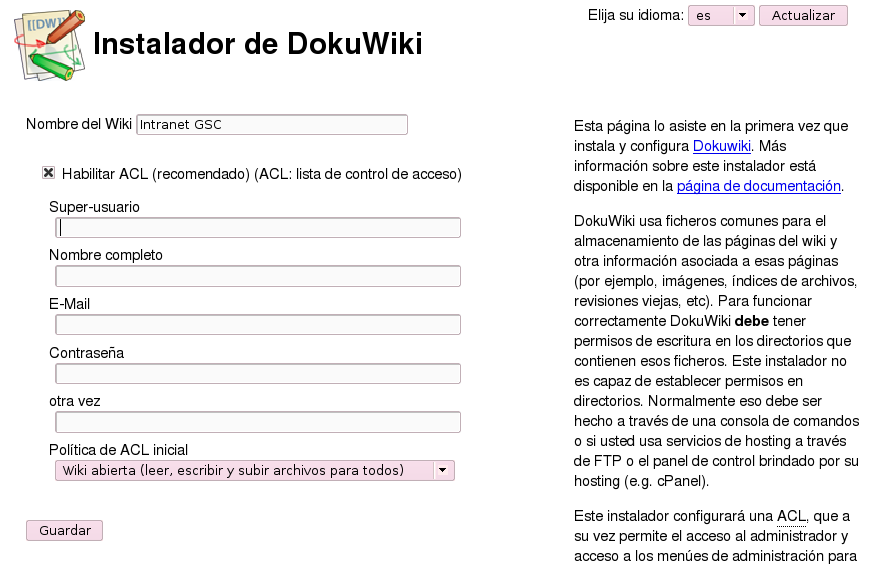
\includegraphics[width=0.8\textwidth]{Utils/instalador_wiki.png}
 % instalacion1.png: 1179668x1179666 pixel, 0dpi, infxinf cm, bb=
 \caption{Instalador web de DokuWiki}
 \label{fig:instalador_wiki}
\end{figure}

\item Una vez finalizada la instalación de DokuWiki, eliminar el archivo \texttt{install.php}:
\begin{listing}[style=consola, numbers=none]
# rm /var/www/dokuwiki/install.php
\end{listing}

\item El wiki ya es accesible de forma local. Para que sea accesible también por otros equipos de la red local habrá que modificar el archivo 000-default para establecer la opción \textit{allow from} a \textit{all}.
\begin{listing}[style=consola, numbers=none]
# nano /etc/apache2/sites-enabled/000-default
\end{listing}
\end{enumerate}

